\section{Binary--mixture confined between two walls}
The first system studied consisted of a binary--mixture of two fluids confined between two walls, corresponding to the physical case of a planar liquid sandwiched between two plates.
The fluid was prepared from a face--centered cubic lattice of spacing $1.64414\ \sigma$ under a pressure of $P^{*} = 0.1$ and temperatures of $T^{*} = 0.8$ and $T^{*} = 0.9$, ensuring the system lay within the liquid region of the Lennard--Jones phase--space.\cite{Smit}
The pressure was controlled by applying an external force on one of the confining walls, which were bonded using a harmonic interaction to create a harmonic lattice.

\subsection{Using the Virial stress}\label{VirialStressPiston}
Initially the two systems were equilibrated for $2 \times 10^{6}$ timesteps (of length $\delta t = 0.001\ \tau$) which was sufficient to create the uniform number density consistent with a fluid state.
The simulations were then run for a further $40 \times 10^{6}$ timesteps over which period the number--density and Virial stress--tensor were spatially averaged into 400 spatial binds and outputted every timestep.
These values were then time-averaged using a block--length of $10\ \tau$ in accordance with the results of the blocking--analysis described in Section 3.5 to produce profiles for the number--density and $\sigma_{xx}(z^{*})$ at $T^{*} = 0.8$ and $T^{*} = 0.9$, as shown in Figures \ref{PisVirRho} and \ref{PisVirStress}. 
Since the size of the box in the z--direction ($L_{z^{*}}$) varies for different temperatures when the pressure is held constant, the spatial averaging was done using a scaled coordinate $z'$ which corresponds to $z^{*} / L_{z^{*}}$.

\FloatBarrier
\begin{figure*}[h]
\centering
\includegraphics[scale=0.8]{PisVirRho}
\caption{PisVirRho caption goes here.}
\label{PisVirRho}
\end{figure*}

\begin{figure*}[h]
\centering
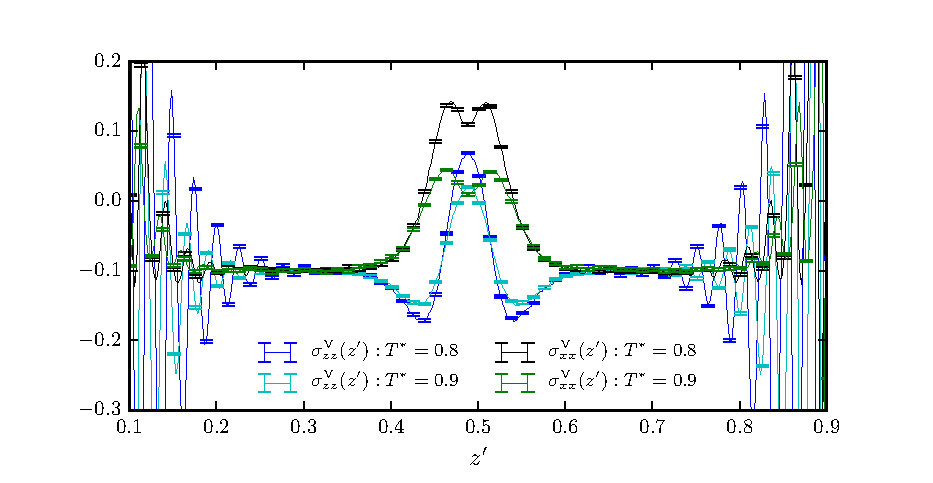
\includegraphics[scale=0.8]{PisVirStress}
\caption{PisVirStress caption goes here.}
\label{PisVirStress}
\end{figure*}

Both the density profile as the stress--profile show the expected features of a binary--mixture. 
Firstly there is a uniform density in the bulk of the fluid and an interfacial region of finite width where the density of one species falls sharply and the density of the other increases.
Close to the walls there are large oscillations in the density which are probably the result of structural layering of the fluid in the vicinity of the harmonically bonded solid walls.
For the stress--profile, we see that the bulk value for the tangential component of the stress is equal to $-P_{\mathrm{ext}}$, corresponding to the hydrostatic pressure of the fluid.
At the interface there is a peak in the tangential stress due to the anisotropy of the intermolecular forces in this region, this peak can be related to the interfacial tension.\cite{Marchand2011}

\FloatBarrier
The time--averaged values for the stress--tensor were then used to estimate the gradient of the stress--tensor with respect to temperature using Equation \ref{FinDiff}, shown in Figure \ref{PisVirForce}.
This gradient shows a clear peak at the interface of the two fluids, corresponding to the expected Marangoni force.
Importantly the force in the bulk of the fluid (far from both the interface and the walls) is zero within statistical error, which agrees with the prediction that there can be no force acting in a bulk fluid as the result of a temperature gradient.
In addition to this, there is also an oscillating force occuring at the surface of the wall which can be interpreted as a thermocapillary force (which notably could also be investigated using this method).
Since we are only interested in simulating the Marangoni effect, these thermocapillary forces were ignored and the central $1/3$ of the force profile was used to create an artifical Marangoni force using a temperature gradient of $\partial T^{*} / \partial x^{*} = 0.001$ and Equation \ref{ForceStressTemp}.

\begin{figure*}[h]
\centering
\includegraphics[scale=0.8]{PisVirForce}
\caption{PisVirForce caption goes here.}
\label{PisVirForce}
\end{figure*}
\FloatBarrier

This artfical body force was applied to an identical system prepared in the same way as before at $T^{*} = 0.85$.
A non-equilibrium simulation was run for $40 \times 10^{6}$ and x--component of the fluid velocity, $v^{*}_{x}$, was spatially and temporally averaged using the same blocking analysis. 
This force profile was then applied as a body force to an identical system prepared at $T^{*} = 0.85$ and the x--component of the velocity was spatially and temporally averaged in an analogous way to the number--density and stress--tensor over $40 \times 10^{6}$ timesteps.
During this simulation the momentum of the walls in the $x$ and $y$ directions was fixed such that they provided a stationary reference point for the fluid.
As a result, the fluid shows a non-slip boundary condition at the walls and thus the walls act to hold the fluid far away from the interface at rest. 

\begin{figure*}[h]
\centering
\includegraphics[scale=0.8]{PisVirFlow}
\caption{PisVirFlow caption goes here.}
\label{PisVirFlow}
\end{figure*}
\FloatBarrier
The flow profile calculated for the fluid in this system is shown in Figure \ref{PisVirFlow}. 
This profile shows a sharp negative peak at the interface of the two fluids indicating a Marangoni flow in the opposite direction to the temperature gradient, as expected.
Furthermore the flow decay away from the interface is essentially linear which is consistent with a Couette flow arising from shear--driven fluid motion.
There is also clearly a net flow of the fluid, suggesting a net force acting on the liquid.
However as was explained in Section \ref{Macroscopic} a temperature gradient should not be able to generate a net flow. 
This is not a problem in this case as the walls which are held stationary act as a momentum sink, providing a friction force on the fluid which allows a steady--state flow to arise under the action of the Marangoni force.
\FloatBarrier

\subsection{Comparing to the Irving--Kirkwood stress}
It is clear from Figure \ref{PisVirRho} that there are significant deviations of the fluid density close at the interface and the walls and that the amount of deviation from the bulk density varies with temperature.
Because of the strong dependence of the Virial stress on the local density of the fluid, there is the potential for these density changes to interfere with the measurement of the Marangoni force.
To verify the significance of these density deviations, the force profile was also calculated using the Irving--Kirkwood formula for the stress--tensor, since this calculates the mometum flux across planes within the fluid and does not depend on the local fluid density.

\begin{figure*}[h]
\centering
\includegraphics[scale=0.8]{PisIKStress}
\caption{PisIKStress}
\label{PisIKStress}
\end{figure*}
In this case the fluids were prepared in the same way as described in Section \ref{VirialStressPiston}.
However since the Irving--Kirkwood stress takes much longer to compute using the post--processing method described in Section \ref{CalcStress}, these simulations were only run at equilibrium for $1 \times 10^{6}$ timesteps, resulting in a greater amount of statistical error.
Over this period, $\sigma^{\mathrm{IK}}_{xx}$ was calculated every 10 timesteps for 400 spatial bins across the z--dimension of the box. 
These were then time--averaged to yield the stress--profiles shown in \ref{PisIKStress}.
\FloatBarrier

\begin{figure*}[h]
\centering
\includegraphics[scale=0.8]{PisIKForce}
\caption{PisIKForce}
\label{PisIKForce}
\end{figure*}
Using the finite difference method this stress--profile was used to calculate the force profile which is compared to that computed from the Virial stress in Figure \ref{PisIKForce}.
Focussing again on only the central $1/3$ of the fluid there is a reasonable good correspondence between the two force profiles as the interfacial peak occurs across the same spatial region and with the same maximum value.
The the most signifcant difference occurs directly at the interface where there is a sharp reduction in the Irving--Kirkwood force, this is probably a result of the reduction in density at the interface affecting the Virial stress more than the Irving--Kirkwood stress.
\FloatBarrier

\begin{figure*}[h]
\centering
\includegraphics[scale=0.8]{PisIKFlow}
\caption{PisIKFlow}
\label{PisIKFlow}
\end{figure*}
An identical non-equilibrium run at $T^{*} = 0.85$ was then performed using the Irving--Kirkwood force profile instead of the Virial force and the flow profile was again calculated.
This was compared to the flow profile calculated using the Virial force as shown in Figure \ref{PisIKFlow}.
The flow profiles plotted show a reasonably good correspondence, especially for the region $z' \leq 0.4$, although the flow from the Irving--Kirkwood force deviates for higher values of $z'$.
In particular the flow from the Irving--Kirkwood force is not a large directly at the interface, as a result of the reduction in the force at this point, and also is assymetric.
Given the symmetry of the system, one would expect the flow profile to be symmetric about the interface and thus this assymmetry is probably a result of the increased amount of noise in the Irving--Kirkwood force profile.
The increase in noise is a consequence of the shorter equilibrium simulation time which was enforced by the high computational cost of the Irving--Kirkwood analysis.

\subsection{Summary}
The finite difference approach for the fluid confined between two walls showed the Marangoni force could be calculated using the Virial stress--tensor and the Irving--Kirkwood stress--tensor.
Both of these methods produced a similar force at the interface of the two fluids although the Irving--Kirkwood stress--tensor gave a reduction in the force calculate directly at the interface.
By applying these force profiles as an applied body force in a non--equilibrium, the Marangoni flow profile was computed and showed a Couette flow.
The flow profile for the Irving--Kirkwood and Virial stress--tensors was very similar although the Irving--Kirkwood profile was not symmetrical, probably due to increased noise in the Irving--Kirkwood force profile.







